
\section{Results}
\label{sec:results}

% \subsection{The Output Plot}
% \label{sub:output}

\begin{figure}[!tb]
	\centering
	\includegraphics[width=\columnwidth]{./output/run-bgdens/bgphotons_1/n1/graph.pdf}
	\caption{
		The beam reconstruction (blue line) of a sumlation run with all the
		expected parameter values. \(E = \SI{1.3}{\giga\electronvolt}\),
		\(\sigma_E = \SI{0.4}{\giga\electronvolt}\), \(\epsilon =
		\SI{1}{\milli\meter\milli\radian}\)
	}
	\label{fig:default}
\end{figure}

\begin{figure}[!tb]
	\centering
	% 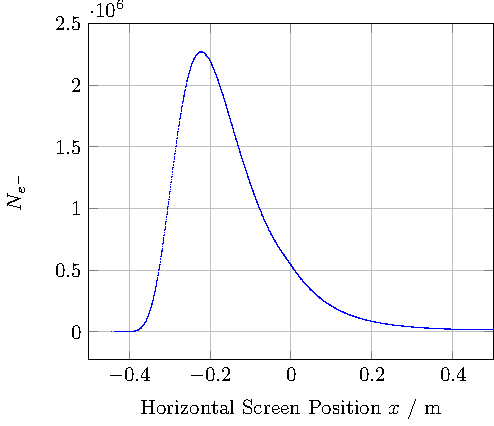
\includegraphics[width=1\linewidth]{./figures/edist.pdf}
	\includegraphics[width=\columnwidth]{./output/run-pespread/pespread_0.01/n1/graph.pdf}
	\caption{
		The beam reconstruction, consistently overestimates the vertical
		beam size. This run used a small percentage energy spread of
		\SI{1}{\percent}. With all other parameters set to their expected
		value.
	}
	\label{fig:yoverestimate}
\end{figure}


Along with the \(\chi^2\) minimised parameter values of the fit, each simulation
generated a plot, showing the simulated, measured and fitted vertical beam size
functions as a function of horizontal position \(x\) on the screen.
Figure~\ref{fig:default} is the output of a run with all parameters set to their
expected values. At these values, the measured beam sizes and the fitted
Figure~\ref{fig:yoverestimate} is an output plot for a run with a small
(\SI{1}{\percent}) energy spread. The solid black line is the shape of the
simulated electron beam that hits the screen, the black points show the
simulated measurements of the RMS width of the fitted Gaussian for each vertical
strip of pixels. The blue dashed line is the beam size function fitted to the
points.

\subsection{Binning errors}

After the investigation of multiple experimental parameters, the emittance
measurement consistently converged to a value \num{1e-8} larger than the input
emittance. The reason for this systematic error was found to be due to the
discretization of the beam hitting the screen meaning that the measurement of
the vertical beam size was consistently overestimated. Since the electrons in
each pixel are not uniformly distributed but rather more densely distributed
closer towards the mean value, giving rise to a systematic overestimation of the
vertical beam size of up to two times the vertical size of the pixel. This
effect can be seen most clearly when a very small energy spread was used as can
be seen in Figure~\ref{fig:yoverestimate}, where the measured beam heights are
consistently larger than the actual beam height.

This systematic error is displayed in subsequent plots as a blue line, where the
red line shows the true beam emittance and the blue line represents where the
emittance measurement should be taking into account this error.

\subsection{Energy Spread}

\begin{figure}[!tb]
	\centering
	% 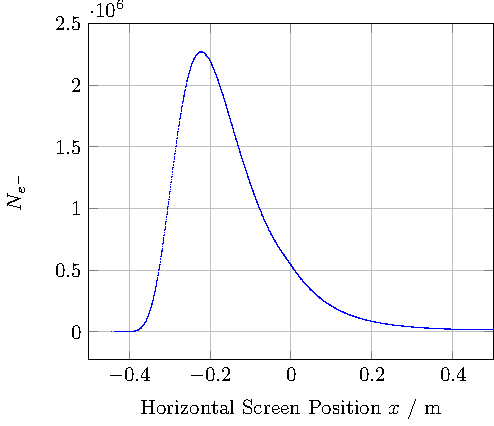
\includegraphics[width=1\linewidth]{./figures/edist.pdf}
	\includegraphics{./output/run-pespread/emit_vs_pespread.pdf}
	\caption{
		Plot of the simulated emittance measurement against the percentage
		spread of the beam energy, showing emittance measurements becoming
		unreliable at percentage energy spreads below \SI{2}{\percent}.
	}
	\label{fig:emit_pespread}
\end{figure}

\begin{figure}[!tb]
	\centering
	% 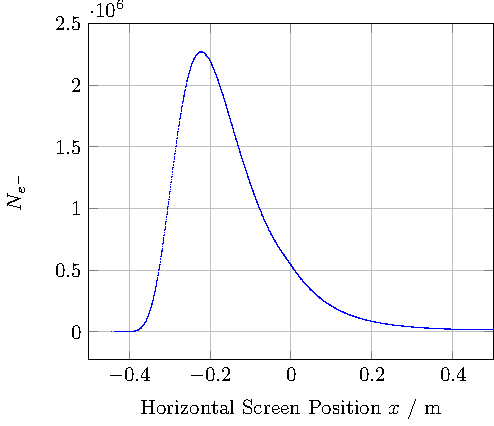
\includegraphics[width=1\linewidth]{./figures/edist.pdf}
	\includegraphics{./output/run-pespread/emitperr_vs_pespread.pdf}
	\caption{
		Plot of the simulated emittance measurement errors against the
		percentage spread of the beam energy, showing an exponential increase in
		the spread of the errors as the percentage error spread is narrowed.
	}
	\label{fig:emitperr_pespread}
\end{figure}


Initially, the mean energy of the beam and energy spread of the beam were tested
independently. Simulations for all combinations of the following energies \(E
\in \left\{ 0.5, 1, 1.3, 2.0, 3.0 5.0\right\} \) and the following energy
spreads \(\sigma_E \in \left\{ 0.01, 0.1, 0.3, 0.4 \right\}\) were run.  These
energies and energy spreads were chosen such that at least one full standard
deviation of the beam hit the screen. As Figure~\ref{fig:eofx} shows, the range
of energies that hit the screen for this setting of the dipole and quadrupole,
is from \SIrange{\sim0.28}{6}{\giga\electronvolt}.
% TODO what is the dipole set to?
% TODO dipole adjustable so could have larger energies?

The smaller the energy spread of the beam the smaller the spread of the beam
across the screen. Figure~\ref{fig:yoverestimate} is a plot showing the full
spread of the beam across the screen for a beam energy spread of
\SI{1}{\percent}. The fewer vertical beam measurements that the function is able
to fit to, the larger the errors of fitting will be, so the relationship between
the errors of the measured emittance and the energy spread in
Figure~\ref{fig:emit_pespread} is the expected result. The expected energy
spread, \SI{0.4}{\giga\electronvolt}, translates to a percentage energy spread
of \SI{30}{\percent} at the expected beam energy of
\SI{1.3}{\giga\electronvolt}. By this point, the error on the measurement of the
emittance has converged to less than a \SI{1}{\percent}.

Plotting the absolute simulated measurement error against the percentage energy
spread in Figure~\ref{fig:emit_pespread} it is clearer the manner in which the
errors blow up for lower energy spreads. 
% This was not the expected result. % Should I say this?
For lower energy spreads, all measurement errors were expected to increase
exponentially.  However this is not the case, but rather, the \emph{spread} of
measurement errors increased exponentially, meaning that may measurement errors
are still only a few percent of the measurement. This behaviour reflects how the
errors for the background noise were calculated; the error associated with the
background photons for each pixel is set to the square root of the number of
background photons. This means the fewer the number of incident background
photons the screen, the smaller the error. However, the error in the uncertainty
of the measurement of the background was not taken into account then scaling the
raw signal back into the real shape. This extra error arises from the
uncertainty in the measurement of the background photon density when there is no
accelerated election beam. To take this into account, this error must be added
in quadrature to each pixel.

The upper ranges of this energy spread may also be investigated, however, this
is less of a priority. Percentage energy spreads up to \SI{80}{\percent} were
investigated without signs of alterations to the measured emittance of emittance
measurement. It is expected that as the beam energy moves outside the
\SIrange{0.28}{6}{\giga\electronvolt} range, emittance measurements will become
more erroneous since most of the beam will not hit the screen.

\subsection{Input Emittance}

\begin{figure}[!tb]
	\centering
	\includegraphics{./output/run-inemit/emitr_vs_inemit.pdf}
	\caption{
		Plot of the ratio between the measured and true emittances of the beam
		against the true emittance of the beam.
		% , showing good measurements of the emittance below an emittance of
		% \SI{e-5}{\meter\radian} and a large underestimation of the emittance
		% for larger emittances.
		The blue line is the expected measurement value when taking into account
		the systematic overestimation due to discrete bins.
	}
	\label{fig:emitr_inemit}
\end{figure}

% \begin{figure}[!tb]
% 	\centering
% 		\centering
% 		\includegraphics{./output/run-inemit/emitrperr_vs_inemit.pdf}
% 		\caption{
% 		}
% 		\label{fig:emitrperr_inemit}
% \end{figure}

\begin{figure}[!tb]
	\centering
	\includegraphics[width=\columnwidth]{./output/run-inemit/emit_7e-5/n1/graph.pdf}
	\caption{
		Beam reconstruction for a large beam emittance of \SI{7e-5}{\meter\radian}
		showing the underestimation of the measured vertical beam sizes.
	}
	\label{fig:large_emit}
\end{figure}

Since the emittance is the parameter required to be measured, a reasonably large
region around the expected emittance should give precise emittance measurements.
The input beam emittance range tested was from \SIrange{1e-7}{1e-4}%
{\meter\radian} as shown in Figure~\ref{fig:emitr_inemit}.
% , where all other parameters kept constant between each run.

\subsection{Background Photons}


\begin{figure}[!t]
	\centering
	\includegraphics{./output/run-bgdens/emit_vs_bgdens.pdf}
	\caption{
	}
	\label{fig:emit_bgdens}
\end{figure}

% \begin{figure}[!t]
% 	\centering
% 	\includegraphics{./output/run-bgdens/emitperr_vs_bgdens.pdf}
% 	\caption{
% 	}
% 	\label{fig:emitperr_bgdens}
% \end{figure}

\begin{figure}[!tb]
	\centering
	\includegraphics[width=\columnwidth]{./output/run-bgdens/bgphotons_1e4/n6/graph.pdf}
	\caption{
		Beam reconstruction for a large background.
	}
	\label{fig:large_bg}
\end{figure}



